\chapter{Best Practices beim Arbeiten mit Polymer}\label{best-practices-beim-arbeiten-mit-polymer}

In den vorherigen Kapiteln wurde gezeigt, welchen Mehrwert Polymer für die Entwickler bringt und wie die Library eingesetzt wird. In diesem Kapitel werden in Abschnitt \ref{ui-performance-patterns} einige \ac{UI}-Performance-Patterns für eine möglichst performante Applikation sowie in Abschnitt \ref{gesture-system} das Gesture-System erläutert. Abschnitt \ref{a11y---barrierefreiheit-in-polymer} erläutert die von Polymer bereitgestellten Mittel zum Entwickeln einer möglichst barrierefreien Applikation.


\section{UI-Performance-Patterns}\label{ui-performance-patterns}

Applikationen und Webseiten in dem modernen Web müssen möglichst schnell Laden sowie ein flüssiges Arbeiten ermöglichen, damit sie von den Benutzern akzeptiert und genutzt werden. In Abbildung \ref{fig:vwdbbul} wird deutlich, dass Applikationen mit einer Ladezeit von ca. 1000 Millisekunden oder mehr sich negativ auf die Zufriedenheit der Nutzer auswirken \cite{citeulike:13262776}.

\begin{figure}[htbp]
 \centering
 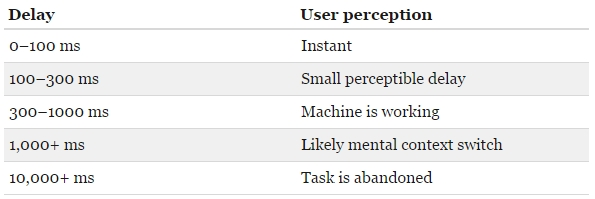
\includegraphics[width=11cm,keepaspectratio]{kapitel6/bilder/1-performance-user-perception-reaction-times}
 \caption{Verschiedene Wahrnehmung der Benutzer bei unterschiedlichen Ladezeiten}
 \label{fig:vwdbbul}
\end{figure}


\subsection{Ladezeiten und initiales Rendern optimieren}\label{ladezeiten-und-initiales-rendern-optimieren}

Ohne ein besonderes Augenmerk auf die Performance zu werfen, bleibt die Seite oder die Applikation beim initialen Laden sehr lange weiß und der Benutzer sitzt vor einem weißen Bildschirm. Wenn alle Ressourcen fertig geladen wurden, wird der Inhalt dann plötzlich und unerwartet eingeblendet. Das erste blockierende Element sind bereits die webcomponents.js Polyfills, da diese in einem \texttt{\textless{}script\textgreater{}}-Tag stehen und somit sequenziell geladen werden müssen und die Ladezeit verlängern. Dies kann jedoch verhindert werden, indem dem Tag das \texttt{async}-Attribut hinzugefügt wird \texttt{\textless{}script\ src=\dq webcomponents.js\dq\ async\textgreater{}\textless{}/script\textgreater{}}, alle anderen Ressourcen können dann asynchron geladen werden und die Applikation muss nicht auf die Polyfills warten. Um die Ladezeit weiter zu verkürzen, kann mittels einer JavaScript-Überprüfung ermittelt werden, ob die Polyfills optional geladen werden müssen (Lazy Load) wenn diese vom Browser nicht unterstützt werden (siehe Listing \ref{bfd}).

\lstinputlisting[language=JavaScript,label=bfd,caption=Browser-Feature-Detection]{kapitel6/listings/1-1.js}

Neben den Polyfills blockieren importierte \ac{HTML}-Dateien, also andere Komponenten, zwar nicht das Laden der Applikation, jedoch dessen Rendern, da diese selbst wiederum sowohl \texttt{\textless{}script\textgreater{}}-Tags als auch Stylesheets beinhalten. Diese blockieren ebenso das Rendern der Webseite, da der Browser die importieren \ac{CSS}-Dateien erst parsen muss. Hier kann ebenfalls das \texttt{async}-Attribut gesetzt werden um dieses Problem zu lösen. Somit wird die Webseite sofort nach dem Laden aller Ressourcen gerendert, jedoch auch ohne Anwendung der Style-Regeln. Der hierdurch entstehende \ac{FOUC} muss also manuell verhindert werden, indem grobe Container in einem \texttt{\textless{}style\textgreater{}}-Tag für das ungefähre Aussehen der Applikation definiert werden. Dadurch werden die Komponenten nach und nach in die Container geladen, es wird somit sofort eine Vorschau der Applikation angezeigt und die Applikation schnell geladen \cite{citeulike:13915203}.


\subsection{Optimierungen für eine flüssige Applikation}\label{optimierungen-fuxfcr-eine-fluxfcssige-applikation}

Wie in Abschnitt \ref{shady-dom} gezeigt, implementiert Polymer eine eigene Version des Shadow \ac{DOM}s, den Shady \ac{DOM}, um eine möglichst breite Browserunterstützung zu gewährleisten. Im Gegensatz zum Shadow \ac{DOM}, welcher im Kontext der Browser in der Programmiersprache C++ programmiert ist, ist der Shady \ac{DOM} nur eine in JavaScript programmierte Nachbildung dessen. Somit ist dieser schon auf Plattform-Ebene langsamer. Zusätzlich ist das Scoping sowie das Rendern im nativen Shadow \ac{DOM} einiges schneller. Vor dem Einbinden der Polymer-Library sollte im globalen \texttt{Polymer}-Settings-Objekt die Property \texttt{dom} auf den Wert \texttt{'shadow'} gesetzt werden. Polymer überprüft daraufhin, ob der Browser das Shadow \ac{DOM} unterstützt.

Um eine schnelle Reaktionszeit der App zu gewährleisten, sollten statt Click-Events immer die Touch-Events verwendet werden (siehe Abschnitt \ref{gesture-system}), da Click-Events auf mobilen Geräten eine Zeitverzögerung von 300 Millisekunden haben, bevor diese tatsächlich abgefeuert werden. Dies wird von den Browserherstellern so implementiert, da die Browser bei Click-Events zu erst prüfen müssen, ob das Event Teil eines Doppel-Taps ist, was einen Zoom auslösen würde.

Darüber hinaus sollten nicht benötigte Elemente nur dann tatsächlich gerendert werden, wenn diese auch wirklich im Viewport des Browsers zu sehen sind (Lazy Render). Wird dies nicht gemacht, werden alle Elemente beim initialen Laden der Seite gerendert, was die Applikation bei mehreren Tausend Elementen sehr träge machen kann. So setzt beispielsweise die \texttt{\textless{}iron-list\textgreater{}}-Komponente von Polymer diese Technik um, indem es nur die Elemente in das \ac{DOM} lädt, welche aktuell sichtbar sein müssen. Ebenso wird das lokale \ac{DOM} des \texttt{dom-if}-Template \texttt{\textless{}template\ is='dom-if'\ if='\{\{open\}\}'\textgreater{}} nur dann generiert und gerendert, wenn das Element aktiv ist, also wenn \texttt{open} den Wert true annimmt. Dies kann unter Anderem bei Dropdown Elementen oder Akkordeon-Menüs umgesetzt werden. Um zu prüfen, wie viele Polymer Komponenten aktuell auf der Seite im \ac{DOM} stehen und Informationen über dessen Performance zu erhalten, stellt Polymer die Erweiterung ``Polymer DevTools Extension'' für den Chrome-Browser zur Verfügung \cite{citeulike:13915202}.


\section{Gesture-System}\label{gesture-system}

Wie bereits in dem vorangegangenen Abschnitt \ref{ui-performance-patterns} angeschnitten wird, sind flüssige Reaktionen auf Aktionen der Benutzer sehr wichtig für gute Applikationen. Um den Umgang mit Input auf verschiedenen Devices zu vereinfachen, stellt Polymer das Gesture-System bereit \cite{citeulike:13915222}. Dieses vereinheitlicht die diversen Eingabemöglichkeiten von Desktops, Smartphones bzw. Tablets und Uhren, welche sich mit Maus und Touch unterschiedlich verhalten. Statt dass Entwickler beide Eingabearten gesondert implementieren müssen, kümmert sich Polymers Gesture-System automatisch darum, indem es die Events von Maus und Touch in 4 einheitliche, für alle Plattformen gleiche, vereint. Hierbei handelt es sich um die Events \texttt{down}, \texttt{up}, \texttt{tap} und \texttt{track}, welche konsistent auf Touch- und Klick-Umgebungen ausgelöst werden und statt den spezifischen Klick- und Touch-Event-Gegenstücken benutzt werden sollten. Um ein Element auf eines der Touch-Events hören zu lassen, kann entweder die imperative oder die deklarative Methode zum Hinzufügen von Events gewählt werden (siehe Abschnitt \ref{events}). Die Events können dem Polymer-Prototyp in dem \texttt{listeners}-Objekt hinzugefügt werden, wie anhand des Beispiels im folgenden Abschnitt unter \ref{beispiel-einer-barrierefreien-komponente} verdeutlicht wird.


\subsection{Down und Up}\label{down-und-up}

Die \texttt{down}- und \texttt{up}-Events werden ausgelöst, wenn der Finger oder die Maus auf das Element drückt oder es loslässt. Sie bilden die einfachsten Gesten des Gesture-Systems, sind aber bei den meisten Anforderungen ausreichend. Diese Events können beispielsweise dazu eingesetzt werden, um zu visualisieren, welches Element gerade berührt oder geklickt wird. Ohne die \texttt{down}- und \texttt{up}-Events müssten die 4 nativen Events \texttt{touchstart}, \texttt{touchend}, \texttt{mousedown} und \texttt{mouseup} implementiert werden. Dabei hören die Touch-Events nur auf das berührte Element, die Maus-Events ändern ihr Ziel beim Bewegen des Mauszeigers, weshalb auf das gesamte Dokument gehört werden muss um auf das \texttt{mouseup}-Event zu warten, was besonders beim Scrollen zu Komplikationen führen kann. Mit Polymer sind hierfür nur die beiden Events \texttt{down} und \texttt{up} notwendig, wie in Listing \ref{pedu} dargestellt.

\lstinputlisting[language=JavaScript,label=pedu,caption=Polymer Events \texttt{down} und \texttt{up}]{kapitel6/listings/1-2.js}


\subsection{Tap}\label{tap}

Das \texttt{tap}-Event verbindet die \texttt{down}- und \texttt{up}-Events und stellt ein Event für das Auswählen und Drücken eines Elements auf allen Devices dar. Es funktioniert dabei gleich für Maus und Touch, wobei sich das Gesture-System intern um die Plattform-Unterschiede kümmert. Das \texttt{tap}-Event ist das am meisten benutzte Event, da die häufigsten Aktionen der Benutzer der \texttt{tap} bzw. der \texttt{click} sind.


\subsection{Track}\label{track}

Das \texttt{track}-Event ist eine Erweiterung des \texttt{tap}-Events und wird ausgelöst, wenn der Finger oder die Maus beim Drücken eines Elements bewegt wird. Es kommt bei allen Aktionen zum Einsatz, bei denen Drag'n'Drop benötigt wird. Drag'n'Drop kann bei der Maus auf native Weise mit der \ac{HTML}5-\ac{API} realisiert werden, jedoch haben viele Plattformen wie Smartphones oder Uhren Touch-Events, wofür die \ac{API} nicht ausgelegt ist. Dadurch wird das gewünschte Verhalten nicht immer erreicht und ist nur kompliziert manuell zu implementieren. Das \texttt{track}-Event soll hier Abhilfe schaffen und das Drag'n'Drop einfacher relaisierbar machen, wobei auf einige Punkte geachtet werden muss.

Werden Elemente mit dem \texttt{track}-Event-Listener ausgestattet, so verhindern diese standardmäßig das Scrollen, da bei Touch-Geräten zwischen Scrollen und Draggen unterschieden werden muss. Beim Initialisieren des Elements muss anschließend die Scroll-Funktion mittels \texttt{this.setScrollDirection(direction,\ node);} wiederhergestellt werden. Wird für den Parameter \texttt{direction} der wert \texttt{'y'} angegeben, so kann über dem Element auf der vertikalen Achse gescrollt werden, wobei das Draggen des Elements in horizontaler Achse möglich ist. Für den \texttt{node}-Parameter wird hier standardmäßig \texttt{this} übergeben, also das auf \texttt{track} zu überwachende Element. Wird das \texttt{track} -Event registriert, so kann es auf 3 verschiedene Status aufgeschlüsselt werden: \texttt{start} \texttt{track} und \texttt{end}. Für jeden Status kann dann das entsprechend gewünschte Verhalten definiert werden.


\section{A11y - Barrierefreiheit in Polymer}\label{a11y---barrierefreiheit-in-polymer}

\begin{quote}
The Web is an increasingly important resource in many aspects of life: education, employment, government, commerce, health care, recreation, and more. It is essential that the Web be accessible in order to provide equal access and equal opportunity to people with disabilities. An accessible Web can also help people with disabilities more actively participate in society. \cite{citeulike:13915280}
\end{quote}

Barrierefreiheit ist besonders im öffentlichen Sektor sehr wichtig, weshalb sie auch bei Polymer eine große Rolle spielt, so werden die gesamten \ac{UI}-Elemente, die Paper Elements, sukzessive barrierefrei neu implementiert. Auch bieten die Iron-Elemente Behaviors für die Barrierefreiheit an (die Accessibility-Behaviors), welche von Custom Elements importiert werden können und das Programmieren von barrierefreien Elementen vereinfachen. Wenn Barrierefreiheit komplett unabhängig von Behaviors erreicht werden soll, bietet sich das Polymer \texttt{hostAttributes}-Objekt an (siehe Abschnitt \ref{das-hostattributes-objekt}). Um die Applikation auf verschiedene Faktoren, welche nachfolgend erläutert werden \cite{citeulike:13915273}, bezüglich Barrierefreiheit zu überprüfen, bietet Polymer das Plugin ``Accessibility Developer Tools'' für den Chrome-Browser an. Dieses weist auf verschiedene Probleme bezüglich der Barrierefreiheit einer Webseite hin, bietet einen erweiterten Inspector für Accessibility-Eigenschaften von Elementen an und kann diverse Tests ausführen, um die Applikation zu analysieren.


\subsection{Fokus / Tastatur}\label{fokus-tastatur}

Der erste Punkt, der eine barrierefreie Applikation auszeichnet, ist deren Bedienbarkeit mit einer Tastatur. So müssen alle Elemente, die eine Interaktion erlauben, mit der Tastatur mittels der Tab- oder den Pfeil-Tasten erreichbar sein. Dies muss gewährleistet werden, falls die Benutzer nicht in der Lage sind eine Maus zu benutzen, oder falls sie nur eine Tastatur benutzen wollen. Um dies zu erreichen, kann das \texttt{tabindex}-Attribut deklarativ für die Elemente definiert werden. Es kann dabei 3 verschiedene Werte annehmen:

\begin{itemize}
\item
  -1, es kann fokussiert werden, aber nicht in einer speziellen
  Reihenfolge im Kontext der umliegenden Elemente
\item
  0, das Element kann in der normalen Reihenfolge des \ac{DOM}s fokussiert
  werden
\item
  \textgreater{} 0, das Element kann in einer selbst definierten Reihenfolge fokussiert
  werden
\end{itemize}

Der Wert \texttt{\textgreater{}\ 0} sollte allerdings im lokalen \ac{DOM} einer Komponente vermieden werden, da nicht vorhersehbar ist, in welcher Reihenfolge das Element auf der einbindenden Webseite zum Einsatz kommt. Alternativ zu der deklarativen Definition des \texttt{tabindex}-Attributs kann es auch in Polymers \texttt{hostAttributes}-Objekt definiert werden, wie im Beispiel einer barrierefreien Komponente in Zeile 15 dargestellt. Nachdem gewährleistet wird, dass das Element mit der Tastatur erreichbar ist, muss dies visuell dargestellt werden. Hierfür kann in den Styles des Elements die Pseudoklasse \texttt{:focus} definiert werden, wie im Beispiel einer barrierefreien Komponente in Zeile 5, oder alternativ das Behavior \texttt{PaperInkyFocusBehavior} dem Element hinzugefügt werden. Muss das Element nun eine Interaktion mit einer bestimmten Taste bereitstellen, so bietet Polymer hierfür das Iron Element \texttt{iron-a11y-keys-behavior} an, welches ein Mixin für Tastatur-Interaktionen darstellt. Es abstrahiert mit einer einfachen Syntax die Unterschiede der Implementierungen von Tastatureingaben der verschiedenen Browser.


\subsection{Semantik}\label{semantik}

Der zweite Punkt ist der korrekte Einsatz der \ac{HTML}-Elemente innerhalb der eigenen Komponenten. So bietet \ac{HTML} über 100 Elemente an, mit denen der Inhalt semantisch strukturiert werden kann. Benutzer mit eingeschränktem Sehvermögen benutzen häufig unterstützende Technologien wie Screenreader, welche Benutzern den Inhalt der Webseite vorlesen. Wird die Webseite nun aus nur 2 unterschiedlichen \ac{HTML}-Tags aufgebaut, z.B. dem \texttt{\textless{}div\textgreater{}}- oder \texttt{\textless{}span\textgreater{}}-Tag, kann der Benutzer sich nicht in der Webseite orientieren. Die Screenreader oder andere \ac{AT} legen hierbei für jedes Element einen Accessibility-Node im Accessibility-Tree an \cite{citeulike:13915306}. Dieser Knoten kann die \ac{ARIA}-Attribute \texttt{role}, \texttt{value}, \texttt{state} und \texttt{properties} haben, welche von Custom Elements deklarativ definiert werden sollten. Die entsprechenden Werte werden für die nativen \ac{HTML}-Elemente vom \ac{W3C} definiert. Ebenso wie der \texttt{tabindex} können die \ac{ARIA}-Attribute im \texttt{hostAttributes}-Objekt definiert werden, wie im Beispiel einer barrierefreien Komponente in Zeile 16. Wenn der Screenreader ein ihm unbekanntes Element findet und diese Attribute nicht definiert sind, wird standardmäßig die Rolle \texttt{group} angenommen, beim Vorlesen des Elements bekommt der Benutzer also nur \texttt{group} zu hören und weiß somit nicht, was das Element semantisch darstellt. Falls das Custom Element keinen Text beinhalten, keine sichtbare Beschreibung hat oder nur als Interaktions-Mittel bezüglich eines anderen Inhaltes dienen sollte, wie z.b. eine Checkbox oder ein Input-Feld, ist es wichtig, die Attribute \texttt{aria-label} oder \texttt{aria-labelledby} zu definieren, welche jenen Inhalt definiert, wie Beispiel einer barrierefreien Komponente in Zeile 9 dargestellt.


\subsection{Flexibles UI}\label{flexibles-ui}

Der letzte Punkt ist das Erstellen einer \ac{UI}, welche sich flexibel an die Bedürfnisse der Benutzer anpassen lässt, oder für Benutzer mit einer Farbschwäche angepasst ist. So sollten Farben nicht als einziges Medium zum Übertragen von Informationen dienen, stattdessen sollte eine weitere farbunabhängige Darstellung gewählt werden, wie beispielsweise ein Hinweistext bei einem falsch ausgefüllten Input-Feld. Abgesehen von Farbtönen können Benutzer auch Probleme mit der Farbintensität haben, verschiedene Grautöne könnten somit nicht mehr unterschieden werden. Deshalb sollte immer ein ausreichend großer Kontrast zwischen der Darstellung der Information und dem Hintergrund gewählt werden.

\begin{quote}
Contrast (Minimum): The visual presentation of text and images of text has a contrast ratio of at least 4.5:1` \cite{citeulike:13915310}
\end{quote}

Darüber hinaus müssen Benutzer mit einer schwachen Sehstärke die Webseite unter Umständen vergrößern können, um sie lesen zu können. Es sollte deshalb immer gewährleistet werden, dass die Seite auch bei einem Zoom-Faktor größer 100 korrekt dargestellt wird.


\subsection{Beispiel einer barrierefreien Komponente}\label{beispiel-einer-barrierefreien-komponente}

Das Listing \ref{bebfk} stellt die in diesem Abschnitt erklären Methoden zum Erstellen einer barrierefreien Komponenten dar.

\lstinputlisting[language=HTML,label=bebfk,caption=Beispiel einer barrierefreien Komponente]{kapitel6/listings/1-3.html}
